% =============================================================================
% CAPÍTULO: EVALUACIÓN EXPERIMENTAL DEL SISTEMA
% =============================================================================

Los capítulos anteriores han descrito la arquitectura, los fundamentos teóricos y la
implementación de cada módulo del sistema propuesto. El presente capítulo tiene como objetivo
demostrar empíricamente que el sistema cumple con los requisitos de rendimiento, integridad y
eficiencia planteados para su aplicación en entornos de gestión de tráfico urbano. Para ello,
se presentan los resultados de experimentos controlados ejecutados sobre los dos módulos que
constituyen el núcleo computacional del sistema: traffic-sync, responsable del análisis
de congestión y la optimización semafórica, y traffic-storage, encargado de la
persistencia verificable y descentralizada de datos de tráfico.

Las evaluaciones persiguen cuatro objetivos específicos. En primer lugar, se estudia la
escalabilidad del módulo de análisis y optimización, analizando cómo evolucionan el
tiempo de procesamiento y el consumo de recursos del sistema conforme aumenta el número de
sensores simulados que operan simultáneamente. En segundo lugar, se mide la eficiencia
del subsistema de almacenamiento distribuido, cuantificando las latencias extremo a extremo de
las operaciones de escritura y lectura sobre la capa IPFS--BlockDAG bajo distintas condiciones
de carga vehicular. En tercer lugar, se verifica la integridad de los datos almacenados
mediante verificación criptográfica, comprobando que los registros recuperados desde
infraestructuras descentralizadas conservan fielmente el contenido original. En cuarto lugar,
se contextualiza el desempeño obtenido mediante una comparación con tecnologías
alternativas de almacenamiento distribuido (particularmente con redes blockchain basadas en
Ethereum) con el fin de evidenciar las ventajas operativas de la arquitectura propuesta para
aplicaciones de monitoreo urbano de alta frecuencia. En quinto lugar, se valida el
desempeño del control semafórico jerárquico (optimización de ciclo mediante PSO combinada
con control local Max-Pressure) frente a planes de tiempo fijo de referencia, mediante una
campaña de comparaciones A/B multi-escenario y multi-semilla que permite establecer bajo
qué condiciones de demanda el sistema propuesto supera a la práctica de temporización fija
vigente.

Todos los experimentos se ejecutaron en hardware de consumo estándar, sin requerir
infraestructura especializada, lo que pone de manifiesto la viabilidad del sistema para
despliegues en entornos municipales con recursos computacionales limitados.

Los resultados de escalabilidad de traffic-sync y de eficiencia de traffic-storage
presentados en las Secciones~\ref{sec:experimentos_sync} y~\ref{sec:experimentos_storage}
fueron publicados originalmente en \cite{chilecon2025} y se reproducen aquí como parte de
la evaluación integral del sistema completo, incluyendo el control semafórico jerárquico
descrito en la Sección~\ref{sec:experimentos_control_ab}.

% =============================================================================
\section{Evaluación del módulo traffic-sync}
\label{sec:experimentos_sync}

El módulo traffic-sync constituye el motor analítico del sistema: recibe métricas
de tráfico, clasifica el estado de congestión mediante un sistema de inferencia difusa tipo
Mamdani y calcula las configuraciones óptimas de temporización semafórica mediante el
algoritmo PSO\@. Si bien en la operación actual el módulo procesa un sensor a la vez, la
arquitectura fue diseñada desde el inicio para soportar la evaluación conjunta de múltiples
sensores agrupados por zonas urbanas. Con el fin de anticipar este escenario de uso futuro, en el que los clústeres de semáforos
deberán analizarse en paralelo para lograr una dispersión efectiva del tráfico, se
realizaron pruebas de escalabilidad simulando entre 250 y 2000 sensores emitiendo datos de
forma simultánea.

\subsection{Entorno y Protocolo de Prueba}
\label{subsec:sync_entorno_protocolo}

Los experimentos se realizaron en dos máquinas de cómputo de propósito general,
sin hardware acelerador y sin soporte de red especializada, reflejando las condiciones
típicas de un entorno de desarrollo o despliegue municipal de bajo presupuesto.
La evaluación del módulo traffic-sync se llevó a cabo en una laptop equipada
con un procesador AMD Ryzen~5 5500U (6 núcleos, 12 hilos, frecuencia máxima de 4,05~GHz),
7,1~GB de memoria RAM disponible y sistema operativo Ubuntu~24.04~LTS\@.
La evaluación del módulo traffic-storage, que requería conectividad real con
servicios distribuidos externos, se realizó en un equipo con procesador AMD Ryzen~7 3700U
(4 núcleos, 8 hilos, frecuencia base de 2,3~GHz), 9,6~GB de memoria RAM total
(5,9~GB disponibles durante las pruebas), almacenamiento SSD NVMe de 233~GB y
el mismo sistema operativo Ubuntu~24.04.2~LTS\@. Ambas configuraciones corresponden
a hardware de consumo estándar disponible comercialmente, hecho que refuerza la
premisa de diseño del sistema: su operatividad no depende de servidores de alta gama
ni de plataformas en la nube.

\subsubsection{Pila de Software}

El sistema se ejecutó sobre Python~3 utilizando FastAPI como framework para las APIs
RESTful de cada módulo. La interacción con la red BlockDAG se gestionó mediante la
biblioteca Web3.py, mientras que el procesamiento de datos de simulación se apoyó
en las herramientas provistas por SUMO\footnote{\url{https://github.com/eclipse-sumo/sumo}}
a través del protocolo TraCI\@. La capa de almacenamiento en IPFS se implementó
utilizando Pinata\footnote{\url{https://pinata.cloud}} como servicio de nodo gestionado,
con autenticación mediante tokens JWT y un gateway personalizado para las operaciones de
descarga. La validación de esquemas de datos en tiempo de ejecución se realizó mediante
Pydantic, que garantiza la consistencia estructural de los mensajes JSON intercambiados
entre módulos.

\subsubsection{Infraestructura de Red Descentralizada}

Las transacciones de almacenamiento se enviaron a la red \textit{Primordial TestNet},
una red BlockDAG de pruebas con identificador de cadena (Chain ID) 1043, accesible
a través del nodo RPC público https://rpc.primordial.bdagscan.com~\cite{wang2023dag}.
El contrato inteligente TrafficStorage.sol, implementado en Solidity~0.8.19,
se encuentra desplegado en la dirección de contrato
\texttt{\footnotesize 0xC3d520EBE9A9F52FC5E1519f\\17F5a9A01d8ac68f}
de dicha red.
El contrato expone dos funciones principales: \texttt{storeRecord}, que registra un
nuevo CID de IPFS asociado a un identificador de semáforo, una marca de tiempo y un
tipo de dato; y \texttt{getRecord}, que recupera el CID correspondiente a una
consulta determinada. Ambas interactúan con un mapeo anidado indexado por
\texttt{trafficLightId}, \texttt{timestamp} y \texttt{DataType}, cuyo valor
almacenado es el \texttt{CID} correspondiente,
garantizando la unicidad de cada registro y facilitando consultas directas sin
recorridos costosos sobre la estructura de datos del contrato.

La Tabla~\ref{tab:entorno_experimental} resume las especificaciones de ambos entornos
de prueba para facilitar la reproducibilidad de los experimentos.

\begin{table}[htbp]
\renewcommand{\arraystretch}{1.3}
\caption{Especificaciones del entorno experimental}
\label{tab:entorno_experimental}
\centering
\footnotesize
\begin{tabular}{lcc}
\hline
\textbf{Parámetro} & \textbf{Entorno A (traffic-sync)} & \textbf{Entorno B (traffic-storage)} \\
\hline
Procesador         & AMD Ryzen 5 5500U      & AMD Ryzen 7 3700U \\
Núcleos / Hilos    & 6 / 12                 & 4 / 8 \\
Frec. máxima       & 4,05 GHz               & 2,3 GHz (base) \\
RAM disponible     & 7,1 GB                 & 5,9 GB \\
Almacenamiento     & N/A                    & 233 GB SSD NVMe \\
Sistema operativo  & Ubuntu 24.04 LTS       & Ubuntu 24.04.2 LTS \\
GPU                & No utilizada           & No utilizada \\
Red                & Wi-Fi doméstica        & Wi-Fi doméstica \\
\hline
\end{tabular}
\end{table}

Se definieron siete niveles de carga: 250, 500, 1000, 1250, 1500, 1750 y 2000 sensores
simulados. Para cada nivel, se midieron tres métricas: el tiempo total de ejecución del
ciclo de análisis y optimización (en segundos), el uso promedio de CPU durante el procesamiento
(en porcentaje) y el uso de memoria RAM en el punto de mayor carga (en megabytes). Las pruebas
se ejecutaron en el Entorno~A (laptop AMD Ryzen~5 5500U, Ubuntu~24.04~LTS), sin soporte de GPU
y bajo condiciones de red doméstica, reflejando un escenario de despliegue realista en hardware
de bajo costo. Los datos de entrada correspondieron a observaciones sintéticas en el formato
unificado versión~2.0, incluyendo métricas de velocidad promedio, densidad vehicular y número
de vehículos por minuto.

\subsection{Tiempo de Ejecución}
\label{subsec:sync_tiempo}

La Figura~\ref{fig:sync_tiempo} muestra la evolución del tiempo total de ejecución en función
de la cantidad de sensores simulados. Los valores obtenidos, que van desde 15,87~s para
250~sensores hasta 67,59~s para 2000~sensores, evidencian un crecimiento aproximadamente
lineal con una pendiente de $\approx 0{,}034$~s por sensor adicional procesado.
Este comportamiento lineal es altamente favorable: indica que el módulo no incurre en
sobrecarga superlineal a medida que se incrementa la carga de trabajo, y que los tiempos
de respuesta son predecibles y controlables mediante particionamiento horizontal de los
sensores. Para la escala más exigente evaluada (2000 sensores), el ciclo completo de
análisis y optimización se completa en 67,6~s, lo que representa una capacidad de
$\approx 0{,}034$~s/sensor y confirma la viabilidad del módulo para escenarios de
optimización por zonas a escala urbana real.

\begin{figure}[htbp]
\centering
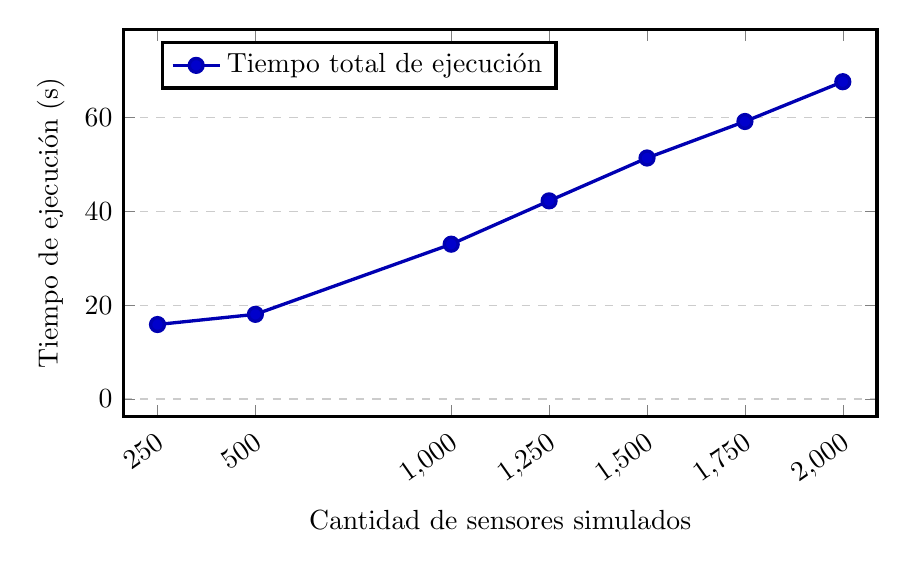
\begin{tikzpicture}
\begin{axis}[
    width=0.92\linewidth,
    height=6.5cm,
    xlabel={Cantidad de sensores simulados},
    ylabel={Tiempo de ejecución (s)},
    ymin=0, ymax=75,
    xtick={250, 500, 1000, 1250, 1500, 1750, 2000},
    xticklabel style={rotate=35, anchor=north east},
    ymajorgrids=true,
    grid style={dashed, gray!40},
    enlargelimits=0.05,
    line width=1.2pt,
    mark size=2.5pt,
    legend style={at={(0.05,0.97)}, anchor=north west},
]
\addplot+[mark=*, color=blue!70!black] coordinates {
    (250,  15.87)
    (500,  18.04)
    (1000, 32.98)
    (1250, 42.21)
    (1500, 51.34)
    (1750, 59.12)
    (2000, 67.59)
};
\addlegendentry{Tiempo total de ejecución}
\end{axis}
\end{tikzpicture}
\caption{Tiempo de ejecución del módulo traffic-sync en función de la cantidad de
sensores simulados. El crecimiento aproximadamente lineal ($\approx$0,034~s/sensor) confirma
la escalabilidad del módulo.}
\label{fig:sync_tiempo}
\end{figure}

\subsection{Uso de CPU y Memoria}
\label{subsec:sync_recursos}

La Figura~\ref{fig:sync_recursos} presenta de forma simultánea el uso promedio de CPU y el
consumo de memoria RAM bajo cada nivel de carga. El comportamiento de ambas métricas
exhibe tendencias en apariencia contrapuestas pero explicables por la naturaleza de la
implementación.

El uso de CPU disminuye progresivamente desde el 72,3\% observado con 250~sensores
hasta el 50,3\% con 2000~sensores. Esta reducción relativa se explica por la naturaleza
de la medición: el porcentaje de CPU se calcula como la razón entre el tiempo de procesador
activo y el tiempo total transcurrido (tiempo de pared). A medida que el volumen de sensores
crece, el tiempo de pared aumenta de forma aproximadamente lineal, mientras que el tiempo
de CPU activo por unidad de trabajo permanece prácticamente constante; el denominador crece
más rápido que el numerador. Entre lotes sucesivos existen períodos de relativa inactividad
(serialización de respuestas, despacho de peticiones HTTP, sobrecarga del intérprete Python)
que incrementan el tiempo de pared sin contribuir proporcionalmente a los ciclos de
procesador. Cabe señalar que tanto el sistema de inferencia difusa Mamdani como el
optimizador PSO son operaciones mayoritariamente CPU-\textit{bound} por unidad; la caída
del porcentaje refleja un efecto de dilución temporal, no una reducción del trabajo
computacional efectivo por sensor.

El consumo de memoria RAM, por su parte, se mantiene estable en el rango de
198--219~MB en todos los escenarios evaluados, creciendo apenas 20,8~MB al pasar de
250 a 2000 sensores (+10,5\%). Esta estabilidad es un indicador clave de la viabilidad del
módulo en dispositivos de recursos acotados, como unidades de cómputo embebido tipo
Raspberry~Pi, donde la memoria disponible suele ser el factor limitante más crítico.

\begin{figure}[htbp]
\centering
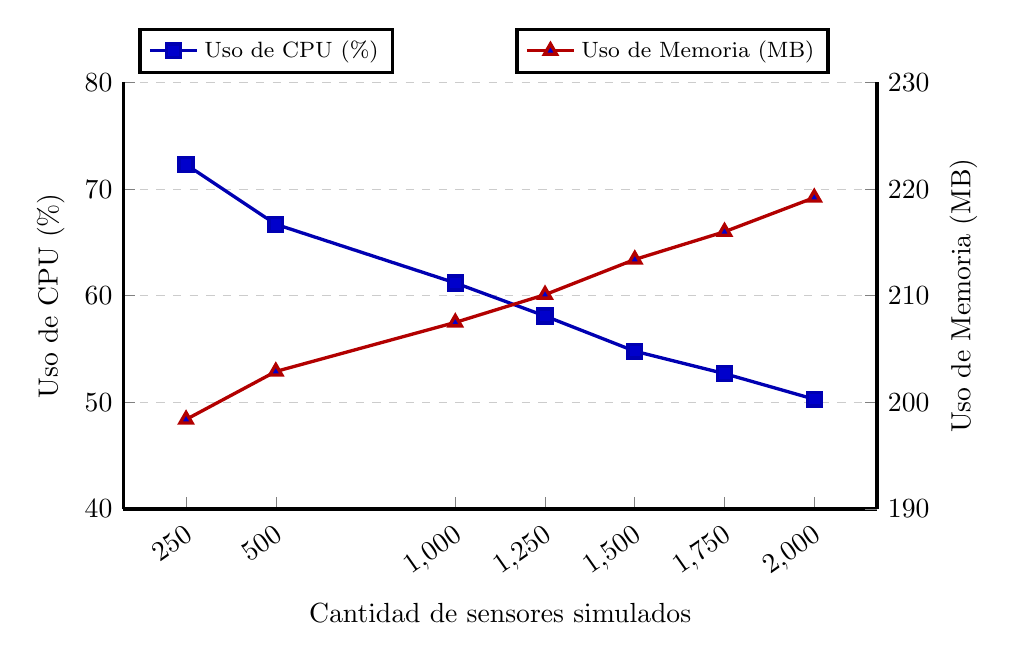
\begin{tikzpicture}
\begin{axis}[
    name=leftaxis,
    width=0.92\linewidth,
    height=7cm,
    xlabel={Cantidad de sensores simulados},
    ylabel={Uso de CPU (\%)},
    ymin=40, ymax=80,
    xtick={250, 500, 1000, 1250, 1500, 1750, 2000},
    xticklabel style={rotate=35, anchor=north east},
    ymajorgrids=true,
    grid style={dashed, gray!40},
    axis y line*=left,
    axis x line*=bottom,
    line width=1.2pt,
    mark size=2.5pt,
    legend style={at={(rel axis cs:0.02,1.02)}, anchor=south west,
                  font=\footnotesize, draw=black, fill=white},
]
\addplot+[mark=square*, color=blue!70!black] coordinates {
    (250,  72.3)
    (500,  66.7)
    (1000, 61.2)
    (1250, 58.1)
    (1500, 54.8)
    (1750, 52.7)
    (2000, 50.3)
};
\addlegendentry{Uso de CPU (\%)}
\end{axis}
%
\begin{axis}[
    width=0.92\linewidth,
    height=7cm,
    ylabel={Uso de Memoria (MB)},
    ymin=190, ymax=230,
    xtick={250, 500, 1000, 1250, 1500, 1750, 2000},
    axis y line*=right,
    axis x line=none,
    line width=1.2pt,
    mark size=2.5pt,
    legend style={at={(rel axis cs:0.52,1.02)}, anchor=south west,
                  font=\footnotesize, draw=black, fill=white},
]
\addplot+[mark=triangle*, color=red!70!black] coordinates {
    (250,  198.4)
    (500,  202.9)
    (1000, 207.5)
    (1250, 210.1)
    (1500, 213.4)
    (1750, 216.0)
    (2000, 219.2)
};
\addlegendentry{Uso de Memoria (MB)}
\end{axis}
\end{tikzpicture}
\caption{Uso promedio de CPU y consumo de memoria RAM del módulo traffic-sync
bajo diferentes cargas de sensores simulados. El CPU disminuye conforme aumenta la
concurrencia; la memoria permanece prácticamente estable en el rango 200--220~MB.}
\label{fig:sync_recursos}
\end{figure}

% =============================================================================
\section{Evaluación del módulo traffic-storage}
\label{sec:experimentos_storage}

El módulo traffic-storage es la capa de persistencia verificable del sistema.
Ante cada reporte de tráfico o resultado de optimización, el módulo sube el contenido en
formato JSON a IPFS y registra el identificador de contenido (CID) resultante en el contrato
inteligente de la red BlockDAG, vinculándolo de forma inmutable al semáforo de origen y la
marca de tiempo correspondiente. La evaluación de este módulo se realizó en dos etapas
complementarias: primero, una medición de métricas de transacción base que caracteriza la
latencia, el costo y el consumo de gas del pipeline completo; y segundo, un protocolo de
prueba por escenarios de tráfico vehicular simulado que valida el comportamiento del sistema
bajo distintas densidades de datos.

% -----------------------------------------------------------------------------
\subsection{Métricas de Transacción Base}
\label{subsec:storage_base}

Para caracterizar el desempeño del pipeline de almacenamiento en condiciones controladas, se
ejecutaron múltiples transacciones reales de subida y descarga sobre un nodo IPFS local
(Kubo) con conexión directa a la red BlockDAG, midiendo cuatro indicadores: tiempo total
de la operación extremo a extremo, tiempo de confirmación en la red BlockDAG, latencia de
red y costo por transacción. La
Tabla~\ref{tab:storage_metricas_base} resume los resultados obtenidos.

\begin{table}[htbp]
\renewcommand{\arraystretch}{1.3}
\caption{Métricas de rendimiento del módulo traffic-storage (IPFS + BlockDAG)}
\label{tab:storage_metricas_base}
\centering
\footnotesize
\begin{tabular}{lcc}
\hline
\textbf{Métrica} & \textbf{Subida (upload)} & \textbf{Bajada (download)} \\
\hline
Tiempo total (s)       & $2{,}47 \pm 0{,}26$ & $1{,}91 \pm 0{,}19$ \\
Confirmación (s)       & $1{,}12 \pm 0{,}14$ & $0{,}98 \pm 0{,}11$ \\
Latencia de red (ms)   & $184 \pm 21$        & $167 \pm 19$        \\
Gas utilizado (upload) & $36.232$--$95.624$\textsuperscript{†}  & ---                 \\
Costo estimado (USD)   & $<0{,}00002$--$<0{,}00005$\textsuperscript{†} & ---       \\
\hline
\end{tabular}
\smallskip

\noindent\textsuperscript{†}~Rango entre datos de tráfico (36.232 unidades,
$<$\$0{,}00002) y resultados de optimización (95.624 unidades, $<$\$0{,}00005);
la descarga usa \texttt{getRecord}, función \textit{view} sin costo on-chain.
Detalle por tipo en Tabla~\ref{tab:storage_gas}.
\end{table}

Los tiempos de confirmación en la red BlockDAG, del orden de 1~segundo, y el costo por
transacción, inferior a \$5 $\times$ 10\textsuperscript{-5}~USD según el tipo de dato
almacenado, confirman la viabilidad del sistema para monitoreo de alta frecuencia;
la comparación con tecnologías alternativas se detalla en la
Sección~\ref{sec:experimentos_comparativa}.

% -----------------------------------------------------------------------------
\subsection{Pruebas con Escenarios de Tráfico Vehicular}
\label{subsec:storage_escenarios}

Con el objeto de evaluar el comportamiento del módulo ante volúmenes de datos representativos
de distintas condiciones operativas reales, se diseñó un protocolo de prueba basado en tres
escenarios de densidad vehicular: bajo, con 30--50 vehículos activos y condiciones
de tráfico fluido; medio, con 80--120 vehículos y tráfico normal en horario diurno;
y alto, con 150--200 vehículos en situación de congestión o pico de demanda.
Los payloads de cada escenario se generaron de forma sintética utilizando el formato unificado
versión~2.0 del sistema, incluyendo métricas por semáforo como vehículos por minuto,
velocidad promedio, tiempo de circulación, densidad y clasificación por tipo de vehículo
(motocicletas, automóviles, autobuses y camiones). A diferencia de las pruebas de la
Sección~\ref{subsec:storage_base}, este protocolo utilizó Pinata como servicio IPFS
gestionado en la nube, lo que introduce latencia adicional por autenticación remota y
transferencia vía gateway externo; esto explica que los tiempos de subida reportados aquí
(6,7--7,3~s) sean superiores a los obtenidos con nodo local (2,47~s). Cada escenario se
ejecutó mediante 5~corridas independientes para obtener estimaciones estadísticamente
representativas de media y desviación estándar.

La Tabla~\ref{tab:storage_escenarios} presenta los tiempos promedio de subida y descarga
para cada escenario, considerando únicamente las corridas con respuesta HTTP~200, que son
aquellas en las que se completó el ciclo completo de almacenamiento y recuperación en
la red BlockDAG\@.

\begin{table}[htbp]
\renewcommand{\arraystretch}{1.3}
\caption{Tiempos de subida y descarga por escenario de tráfico (5 corridas válidas por escenario)}
\label{tab:storage_escenarios}
\centering
\footnotesize
\begin{tabular}{lccc}
\hline
\textbf{Escenario} & \textbf{Corridas válidas} & \textbf{Subida (avg $\pm$ sd, s)} & \textbf{Descarga (avg $\pm$ sd, s)} \\
\hline
Bajo  & 5 & $6{,}725 \pm 1{,}035$ & $1{,}981 \pm 0{,}861$ \\
Medio & 5 & $6{,}896 \pm 0{,}963$ & $1{,}750 \pm 0{,}136$ \\
Alto  & 5 & $7{,}290 \pm 0{,}787$ & $1{,}767 \pm 0{,}174$ \\
\hline
\end{tabular}
\end{table}

La Figura~\ref{fig:storage_escenarios} ilustra gráficamente los tiempos promedio de cada
operación con sus barras de error correspondientes a una desviación estándar. Puede
observarse que el tiempo de subida crece levemente con la densidad vehicular, de
6,725~s en el escenario bajo a 7,290~s en el escenario alto, un incremento del 8,4\%,
mientras que el tiempo de descarga permanece prácticamente estable en todos los escenarios,
con variaciones inferiores a 0,25~s. Este comportamiento confirma que el módulo escala
con el volumen de datos sin comprometer significativamente el rendimiento: el tamaño del
payload influye de forma marginal en la latencia total, que está dominada principalmente
por los tiempos de red y confirmación en la cadena.

\begin{figure}[htbp]
\centering
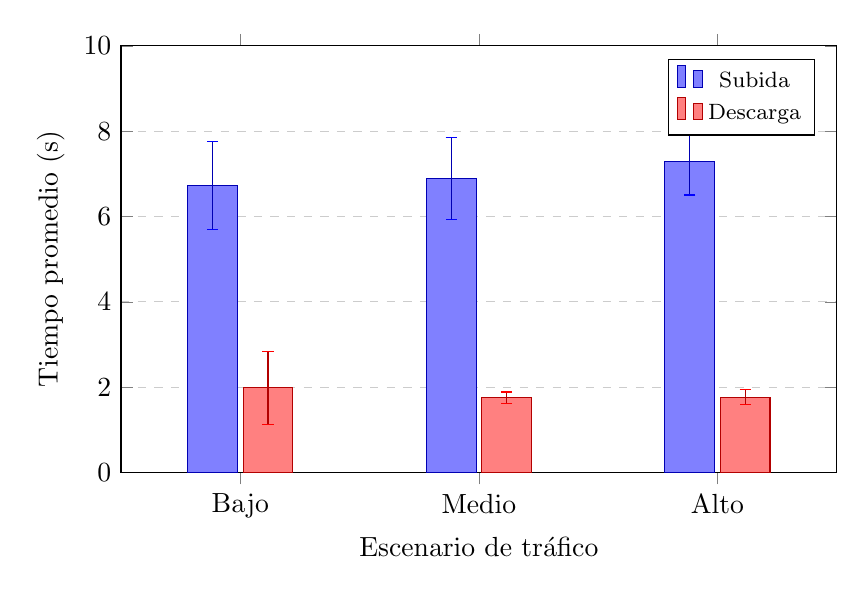
\begin{tikzpicture}
\begin{axis}[
    width=0.88\linewidth,
    height=7cm,
    ybar,
    bar width=18pt,
    symbolic x coords={Bajo, Medio, Alto},
    xtick=data,
    xlabel={Escenario de tráfico},
    ylabel={Tiempo promedio (s)},
    ymin=0, ymax=10,
    ymajorgrids=true,
    grid style={dashed, gray!40},
    legend style={at={(0.97,0.97)}, anchor=north east,
                  font=\footnotesize, draw=black, fill=white},
    error bars/y dir=both,
    error bars/y explicit,
    enlarge x limits=0.25,
]
\addplot+[
    fill=blue!50!white, draw=blue!70!black,
    error bars/.cd, y dir=both, y explicit
] coordinates {
    (Bajo,  6.725) +- (0, 1.035)
    (Medio, 6.896) +- (0, 0.963)
    (Alto,  7.290) +- (0, 0.787)
};
\addlegendentry{Subida}
\addplot+[
    fill=red!50!white, draw=red!70!black,
    error bars/.cd, y dir=both, y explicit
] coordinates {
    (Bajo,  1.981) +- (0, 0.861)
    (Medio, 1.750) +- (0, 0.136)
    (Alto,  1.767) +- (0, 0.174)
};
\addlegendentry{Descarga}
\end{axis}
\end{tikzpicture}
\caption{Tiempos promedio de subida y descarga del módulo traffic-storage por
escenario de tráfico. Las barras de error representan $\pm$1 desviación estándar.
El incremento de latencia de subida entre el escenario bajo y el alto es del 8,4\%.}
\label{fig:storage_escenarios}
\end{figure}

% -----------------------------------------------------------------------------
\subsection{Descomposición del Pipeline de Almacenamiento}
\label{subsec:storage_pipeline}

El tiempo total de una operación de subida no es atómico: comprende varias etapas
secuenciales con latencias propias. El análisis de los registros de ejecución detallados
permite identificar las tres fases que componen el pipeline de almacenamiento. La primera
fase es la subida a IPFS: la serialización del payload JSON, la autenticación
con la API de Pinata y la transferencia del contenido hasta obtener el CID insume
aproximadamente 1,2~s. La segunda fase es la preparación de la transacción
BlockDAG: incluye la verificación del estado del nodo y el balance de la cuenta,
el cálculo dinámico del precio de gas, la obtención del nonce actual y la firma
criptográfica de la transacción; en conjunto, esta fase demanda aproximadamente 2,3~s.
La tercera fase es la confirmación en la red: el tiempo que transcurre desde
el envío de la transacción hasta que es incluida en un bloque minado y confirmada
es de aproximadamente 3,5~s en las pruebas por escenarios. Este valor es superior
al registrado en las pruebas base (1,12~s, Tabla~\ref{tab:storage_metricas_base}),
diferencia atribuible a las condiciones variables de la red BlockDAG pública entre
sesiones de prueba realizadas en distintas fechas.

La Figura~\ref{fig:storage_pipeline} muestra la composición proporcional de estas
etapas para las operaciones de subida y descarga. En el caso de la descarga, el
pipeline se reduce a dos fases: la consulta al contrato inteligente para recuperar
el CID asociado a un semáforo y timestamp determinados (~0,9~s), seguida de la
descarga del contenido desde el gateway de IPFS usando dicho CID (~0,7~s), con
un tiempo total de ~1,6~s.

\begin{figure}[htbp]
\centering
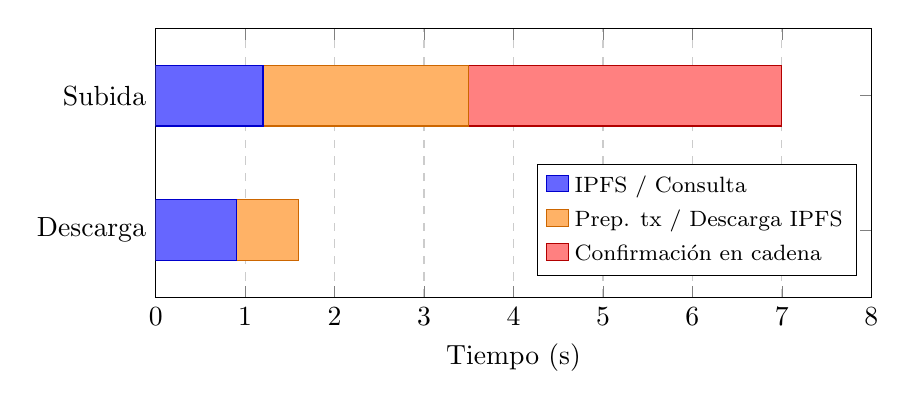
\begin{tikzpicture}
\begin{axis}[
    xbar stacked,
    width=0.88\linewidth,
    height=5cm,
    xlabel={Tiempo (s)},
    symbolic y coords={Descarga,Subida},
    ytick=data,
    xmin=0, xmax=8,
    xmajorgrids=true,
    grid style={dashed, gray!40},
    bar width=22pt,
    legend style={at={(rel axis cs:0.98,0.08)}, anchor=south east,
                  font=\footnotesize, draw=black, fill=white,
                  legend columns=1, row sep=1pt,
                  legend cell align=left},
    enlarge y limits=0.5,
]
\addplot+[fill=blue!60!white, draw=blue!80!black] coordinates {
    (1.2,Subida)
    (0.9,Descarga)
};
\addlegendentry{IPFS / Consulta}
\addplot+[fill=orange!60!white, draw=orange!80!black] coordinates {
    (2.3,Subida)
    (0.7,Descarga)
};
\addlegendentry{Prep. tx / Descarga IPFS}
\addplot+[fill=red!50!white, draw=red!70!black] coordinates {
    (3.5,Subida)
    (0.0,Descarga)
};
\addlegendentry{Confirmación en cadena}
\end{axis}
\end{tikzpicture}
\caption{Desglose del tiempo de ejecución en las operaciones de subida y descarga del
módulo traffic-storage. La confirmación en la red BlockDAG domina la latencia
de subida ($\approx$50\%), mientras que la descarga se completa en $\approx$1,6~s
sin necesidad de esperar confirmación.}
\label{fig:storage_pipeline}
\end{figure}

% -----------------------------------------------------------------------------
\subsection{Verificación de Integridad y Trazabilidad}
\label{subsec:storage_integridad}

Dado que el CID es el resumen criptográfico del contenido (véase la
Sección~\ref{subsec:ipfs_traffic_storage}), la recuperación exitosa del archivo original
constituye por sí misma una prueba de integridad. Esta propiedad fue verificada de forma
experimental durante las pruebas por escenarios:
el contenido descargado en cada corrida produjo consistentemente el mismo resumen
criptográfico, independientemente del momento de ejecución y del escenario de tráfico.
Adicionalmente, el mismo CID fue recuperado en las cinco corridas de cada escenario,
lo que confirma que el contrato inteligente almacena y retorna los metadatos de forma
determinista y reproducible. La Tabla~\ref{tab:storage_evidencias} presenta una muestra
representativa de las transacciones registradas, incluyendo el CID de IPFS y el número
de bloque en que fue confirmada cada operación.

\begin{table}[htbp]
\renewcommand{\arraystretch}{1.3}
\caption{Muestra de transacciones exitosas registradas durante las pruebas}
\label{tab:storage_evidencias}
\centering
\footnotesize
\begin{tabular}{llcc}
\hline
\textbf{Escenario} & \textbf{CID de IPFS (truncado)} & \textbf{Estado HTTP} & \textbf{Bloque} \\
\hline
Bajo  & \texttt{Qmf9gGPs...G3AZox} & 200 & confirmado \\
Medio & \texttt{QmXkDdj8...zHSHR}  & 200 & confirmado \\
Alto  & \texttt{QmUK7Jxz...MDy8}   & 200 & confirmado \\
\hline
\end{tabular}
\end{table}

La trazabilidad de cada operación queda garantizada por el evento RecordStored
emitido por el contrato inteligente en cada transacción exitosa, el cual registra de forma
inmutable el identificador del semáforo, la marca de tiempo, el tipo de dato y el CID
en el historial de la red BlockDAG\@. Este mecanismo permite a cualquier auditor externo
verificar de forma independiente que un dato determinado fue almacenado en un instante
concreto, sin necesidad de confiar en el operador del sistema.

% -----------------------------------------------------------------------------
\subsection{Consumo de Gas y Costos Operativos}
\label{subsec:storage_gas}

El consumo de gas de las transacciones en la red BlockDAG varía según el tipo de dato
almacenado. Las operaciones de almacenamiento de datos de tráfico sin procesar consumen
aproximadamente 36.232 unidades de gas, mientras que las
operaciones de almacenamiento de resultados de optimización,
que incluyen un mayor volumen de campos calculados, consumen aproximadamente
95.624 unidades. La Tabla~\ref{tab:storage_gas} resume el consumo y el costo estimado
en dólares para cada tipo de operación.

\begin{table}[htbp]
\renewcommand{\arraystretch}{1.3}
\caption{Consumo de gas y costo estimado por tipo de operación de almacenamiento}
\label{tab:storage_gas}
\centering
\footnotesize
\begin{tabular}{lcc}
\hline
\textbf{Tipo de dato}         & \textbf{Gas consumido (unidades)} & \textbf{Costo estimado (USD)} \\
\hline
Datos de tráfico (\texttt{Data})         & 36.232 & $< 0{,}00002$ \\
Optimizaciones (\texttt{Optimization})   & 95.624 & $< 0{,}00005$ \\
\hline
\end{tabular}
\end{table}

Incluso para el tipo de operación más costosa, el almacenamiento de resultados de
optimización con 95.624 unidades de gas, el costo por transacción se mantiene por
debajo de \$0{,}00005~USD\@. Considerando una frecuencia de reporte típica de un ciclo
cada 60~segundos por semáforo, el costo anual de almacenamiento on-chain para un
semáforo individual sería inferior a \$0{,}88~USD según las condiciones observadas
durante los experimentos. Sin embargo, esta estimación debe interpretarse con cautela:
los experimentos se realizaron sobre una red BlockDAG pública de pruebas (testnet), cuyo
token no posee valor de mercado real. Los costos en una red de producción (mainnet)
dependerán del precio del token en el momento del despliegue y de la demanda de la red,
por lo que este valor constituye únicamente un orden de magnitud comparativo, no una
proyección de costo operativo real.

% =============================================================================
\section{Comparación con Tecnologías Alternativas}
\label{sec:experimentos_comparativa}

Los resultados experimentales adquieren mayor significado cuando se los sitúa en
relación con las alternativas tecnológicas disponibles para el almacenamiento
distribuido con trazabilidad. Esta sección compara la solución adoptada, IPFS
combinado con una red BlockDAG, frente a la plataforma blockchain de propósito
general más utilizada, Ethereum, tanto desde la perspectiva teórica apoyada en
literatura existente como desde los valores medidos experimentalmente.

\subsection{BlockDAG frente a Ethereum}
\label{subsec:comparativa_blockdag_ethereum}

Las características de ambas plataformas se describieron en el
Capítulo~\ref{sec:decentralized_tech_traffic_storage}; los resultados medidos en este
trabajo, con confirmación en $\approx$1~s y costos inferiores a
\$1{,}2$\times$10\textsuperscript{-5}~USD por transacción, ratifican las ventajas
teóricas de BlockDAG en condiciones de uso real sobre la red Primordial TestNet.
La Tabla~\ref{tab:comparativa_blockchain} sintetiza la comparación desde la perspectiva
del monitoreo urbano de tráfico.

\begin{table}[htbp]
\renewcommand{\arraystretch}{1.3}
\caption{Comparación técnica entre Ethereum y BlockDAG en el contexto de monitoreo
urbano de tráfico. Valores de BlockDAG medidos en Primordial TestNet.}
\label{tab:comparativa_blockchain}
\centering
\footnotesize
\setlength{\tabcolsep}{6pt}
\begin{tabular}{@{}>{\centering\arraybackslash}p{0.34\textwidth}>{\centering\arraybackslash}p{0.31\textwidth}>{\centering\arraybackslash}p{0.31\textwidth}@{}}
\hline
\textbf{Criterio} & \textbf{Ethereum} & \textbf{BlockDAG} \\
\hline
Latencia de confirmación
  & 15--60~s \cite{conoscenti2016blockchain,garay2015backbone}
  & $\approx$1~s (medido) \\
Costo por transacción
  & \$0{,}50--5{,}00~USD \cite{eckermann2021blockchain}
  & $<$\$0{,}00002~USD (medido) \\
Throughput (TPS)
  & 15--30 \cite{buterin2014ethereum}
  & $>$1.000 \cite{sompolinsky2021phantom} \\
Modelo de consenso
  & Proof-of-Stake
  & PoW asíncrono \\
Estructura de datos
  & Cadena lineal
  & Grafo acíclico \\
Contratos inteligentes
  & Maduro (EVM, Solidity)
  & Disponible (EVM-compatible) \\
Escalabilidad
  & Limitada
  & Alta \\
Compatibilidad edge/IoT
  & Baja (nodos pesados)
  & Alta (nodos ligeros) \\
\hline
\end{tabular}
\end{table}

\subsection{Reducción de Latencia respecto a Plataformas Centralizadas}
\label{subsec:comparativa_centralizada}

Más allá de la comparación entre plataformas descentralizadas, la arquitectura
propuesta también supera a las soluciones IoT-cloud centralizadas convencionales
en términos de latencia de persistencia verificable. Los sistemas centralizados
típicos introducen latencias de confirmación de escritura del orden de 3--6~s
cuando incluyen mecanismos de integridad (firmas digitales, logs de auditoría)
\cite{singh2020blockchain,conoscenti2016blockchain},
mientras que la confirmación BlockDAG obtenida en este trabajo alcanzó $\approx$1~s.
Esto representa una reducción de latencia superior al 60\% respecto
a dichos sistemas, con la ventaja adicional de que la inmutabilidad está garantizada
por el protocolo de consenso distribuido, y no por la confianza en un operador
central, y el costo operativo es órdenes de magnitud inferior.

Este conjunto de propiedades, latencia baja, costo insignificante, inmutabilidad
criptográfica e independencia de infraestructura centralizada, posiciona a la
combinación IPFS+BlockDAG como una alternativa técnicamente superior para
aplicaciones de monitoreo urbano con alta frecuencia de reporte y requisitos de
trazabilidad auditables.

% =============================================================================
\section{Evaluación del control semafórico: campaña A/B}
\label{sec:experimentos_control_ab}

Mientras que las secciones anteriores caracterizan el desempeño computacional de los
módulos traffic-sync y traffic-storage de forma aislada, esta sección evalúa el
efecto del control semafórico jerárquico propuesto, PSO de ciclo combinado con
Max-Pressure local, sobre el tránsito vehicular en simulación, en comparación directa
con planes de tiempo fijo de referencia representativos de la práctica vigente.
Esta campaña constituye la validación empírica sobre un mapa real de la ciudad de San
Lorenzo, Paraguay, que \cite{chilecon2025} planteó como trabajo en curso, ejecutada ahora
sobre la versión jerárquica del control (PSO de ciclo por clúster más Max-Pressure local)
en lugar del ajuste directo de tiempos de señal evaluado en aquel trabajo.

\subsection{Diseño experimental}
\label{subsec:control_diseno}

El protocolo de evaluación se basa en comparaciones pareadas A/B: para cada combinación
de un plan fijo de referencia, un escenario de demanda y una semilla aleatoria, se
ejecutan dos corridas de simulación sobre la misma red vial, la misma matriz de demanda
y la misma semilla del motor SUMO, difiriendo únicamente en el mecanismo de control
semafórico. La corrida~A opera con el plan de tiempo fijo de referencia y la corrida~B
con el sistema completo propuesto (PSO de ciclo más Max-Pressure local). La red vial
utilizada corresponde al microcentro de la ciudad de San Lorenzo, con seis intersecciones
semaforizadas cuya lógica de fases fue generada automáticamente mediante la opción
\texttt{--tls.guess} de netconvert. Se consideraron tres planes fijos de referencia,
seis escenarios de demanda y diez semillas aleatorias independientes por celda, lo que
produce $3 \times 6 \times 10 = 180$ comparaciones A/B. Las semillas se generaron
mediante un generador criptográficamente seguro (CSPRNG) y quedaron registradas para
garantizar la reproducibilidad exacta de cada corrida.

\subsection{Escenarios de demanda}
\label{subsec:control_escenarios}

Los seis escenarios evaluados se derivaron de forma determinista, sin componentes
aleatorios, a partir de un mismo archivo base de rutas (\texttt{routes.rou.xml}), de
modo que las diferencias entre escenarios provienen exclusivamente de la manipulación
programática de los volúmenes y patrones de inserción, y no de variabilidad estocástica
adicional. La Tabla~\ref{tab:control_escenarios} resume su definición.

\begin{table}[htbp]
\renewcommand{\arraystretch}{1.3}
\caption{Escenarios de demanda evaluados en la campaña A/B de control semafórico}
\label{tab:control_escenarios}
\centering
\footnotesize
\begin{tabular}{lp{0.72\textwidth}}
\hline
\textbf{Escenario} & \textbf{Definición} \\
\hline
demanda\_baja    & 35\% de la flota vehicular base. \\
demanda\_media   & 65\% de la flota vehicular base. \\
demanda\_alta    & 100\% de la flota vehicular base. \\
demanda\_saturada & 140\% de la flota vehicular base, mediante duplicación intercalada de vehículos. \\
hora\_pico        & Perfil de inserción triangular, con dos tercios de las salidas concentradas
                      en el tercio central de la ventana de simulación. \\
corredor          & Calle dominante con demanda duplicada respecto de la base y calles
                      transversales reducidas al 20\%, dentro de una ventana de 1800~s. \\
\hline
\end{tabular}
\end{table}

\subsection{Planes fijos de referencia}
\label{subsec:control_planes}

Los tres planes fijos de referencia representan puntos distintos del espacio de diseño
de temporización semafórica convencional, desde el reparto normativo igualitario hasta
el residuo de un algoritmo de generación automática de planes. La
Tabla~\ref{tab:control_planes} los resume.

\begin{table}[htbp]
\renewcommand{\arraystretch}{1.3}
\caption{Planes fijos de referencia utilizados en la campaña A/B}
\label{tab:control_planes}
\centering
\footnotesize
\begin{tabular}{lp{0.68\textwidth}}
\hline
\textbf{Plan} & \textbf{Definición y origen} \\
\hline
MOPC 60~s      & Ciclo de 60~s con 25~s de verde por fase, siguiendo el reparto igualitario
                 recomendado por el Manual de Carreteras del Paraguay en ausencia de datos
                 de volumen vehicular por aproximación (sección 113.14.3) \cite{mopc2019manual}.
                 El tiempo perdido por ciclo asociado a este reparto es del 16,7\%. \\
netconvert 90~s & Ciclo de 90~s con 42~s de verde, calculado como el residuo del algoritmo
                 de generación automática de planes de netconvert: el valor por defecto
                 \texttt{tls.cycle.time=90} (\texttt{NBFrame.cpp}, línea~584) y el verde
                 semilla de 31~s (línea~587) se ajustan mediante estiramiento igualitario
                 en \texttt{NBOwnTLDef.cpp} (líneas~803--816), de modo que
                 $31+(90-68)/2=42$. El tiempo perdido por ciclo es del 6,7\%. \\
Ciclo largo 120~s & Ciclo de 120~s con 57~s de verde. El tiempo perdido por ciclo es del 5\%. \\
\hline
\end{tabular}
\end{table}

\subsection{Metodología de evaluación insesgada}
\label{subsec:control_metodologia}

La comparación directa de tiempos de viaje promedio a partir del archivo
\texttt{tripinfo.xml} de SUMO está expuesta a un sesgo de supervivencia: dicho archivo
registra únicamente los viajes completados durante la ventana de simulación, de modo que,
cuando uno de los dos lados de la comparación colapsa parcialmente (los vehículos quedan
atrapados en congestión y no llegan a destino), su promedio de tiempo de viaje se calcula
solo sobre los vehículos rápidos que lograron escapar, produciendo una estimación
artificialmente favorable para el lado colapsado. Para neutralizar este efecto se adoptó
un veredicto compuesto por comparación. En primer lugar, se aplica una guardia de
throughput con autoridad sobre las métricas por viaje: si el número de vehículos que
completan su viaje difiere en más de un 10\% entre las corridas A y B, el veredicto se
determina por throughput, independientemente de lo que indiquen los tiempos de viaje
promedio. En segundo lugar, se incorpora el tiempo total de sistema calculado a partir de
\texttt{summary.xml}, que contabiliza a los vehículos aún circulando o atrapados al cierre
de la ventana de simulación y por lo tanto no hereda el sesgo de supervivencia de
\texttt{tripinfo.xml}. En tercer lugar, se construye evidencia pareada por vehículo,
emparejando cada vehículo por su salida y ruta idénticas en las corridas A y B, sobre la
cual se aplica un test de Wilcoxon de rangos con signo. Se define además una banda de
empate del 2\%, dentro de la cual una comparación se considera neutra en lugar de
favorable o desfavorable, y se registra el número de vehículos nunca insertados en cada
corrida (diferencia entre vehículos cargados y vehículos efectivamente insertados en la
red), indicador adicional de saturación de la demanda de entrada.

\subsection{Resultados globales}
\label{subsec:control_resultados}

Sobre las 180 comparaciones A/B ejecutadas, el sistema propuesto resultó favorable en 140
(77,8\%), con un desglose por plan de referencia de 48/60 comparaciones favorables frente
al plan MOPC~60~s, 46/60 frente a netconvert~90~s y 46/60 frente al ciclo largo~120~s. La
Tabla~\ref{tab:control_favorables_celda} desagrega estos resultados por escenario y
campaña, indicando en cada celda el número de corridas favorables sobre 10 y las medianas
de variación porcentual de throughput ($\Delta$thr) y de tiempo total de sistema
($\Delta$sys). Es importante notar que estas medianas se calculan sobre el total de las
10 corridas de cada celda, incluyendo tanto las favorables como las desfavorables, de
modo de no reintroducir el sesgo de selección que la metodología de la
Sección~\ref{subsec:control_metodologia} busca evitar.

\begin{table}[htbp]
\renewcommand{\arraystretch}{1.3}
\caption{Corridas favorables (de 10) y medianas de variación porcentual de throughput y
tiempo de sistema, por escenario y campaña de comparación}
\label{tab:control_favorables_celda}
\centering
\footnotesize
\begin{tabular}{lccccccccc}
\hline
& \multicolumn{3}{c}{\textbf{MOPC 60~s}} & \multicolumn{3}{c}{\textbf{netconvert 90~s}} & \multicolumn{3}{c}{\textbf{Ciclo largo 120~s}} \\
\textbf{Escenario} & fav. & $\Delta$thr & $\Delta$sys & fav. & $\Delta$thr & $\Delta$sys & fav. & $\Delta$thr & $\Delta$sys \\
\hline
corredor          & 10/10 & +207,5\% & +57,3\% & 10/10 & +159,6\% & +57,7\% & 10/10 & +22,6\% & +28,6\% \\
demanda\_baja      & 9/10  & +5,5\%   & +42,8\% & 8/10  & +10,9\%  & +35,9\% & 8/10  & +14,8\% & +39,2\% \\
demanda\_media     & 9/10  & +51,8\%  & +20,8\% & 9/10  & +25,5\%  & +9,1\%  & 9/10  & +48,6\% & +9,0\% \\
demanda\_alta      & 5/10  & +9,0\%   & +1,9\%  & 5/10  & +7,6\%   & -7,2\%  & 5/10  & +15,4\% & -8,8\% \\
demanda\_saturada  & 8/10  & +46,3\%  & +6,0\%  & 8/10  & +19,6\%  & -5,2\%  & 7/10  & +25,2\% & -7,3\% \\
hora\_pico         & 7/10  & +22,7\%  & +3,0\%  & 6/10  & +15,3\%  & -1,3\%  & 7/10  & +23,8\% & -4,7\% \\
\hline
\end{tabular}
\end{table}

La Figura~\ref{fig:control_favorables} presenta gráficamente el conteo de corridas
favorables por escenario y campaña, mientras que las Figuras~\ref{fig:control_thr} y
\ref{fig:control_sys} muestran las medianas de variación porcentual de throughput y de
tiempo de sistema, respectivamente.

\begin{figure}[htbp]
\centering
\begin{tikzpicture}
\begin{axis}[
    ybar,
    bar width=7pt,
    width=0.95\linewidth,
    height=7cm,
    symbolic x coords={corredor,baja,media,alta,saturada,pico},
    xtick=data,
    xlabel={Escenario},
    ylabel={Corridas favorables (de 10)},
    ymin=0, ymax=11,
    ymajorgrids=true,
    grid style={dashed, gray!40},
    legend style={at={(0.5,-0.22)}, anchor=north, legend columns=3,
                  font=\footnotesize, draw=black, fill=white},
    enlarge x limits=0.12,
]
\pgfplotstableread{datos/favorables.dat}\favtable
\addplot table[x=escenario, y=mopc_60] {\favtable};
\addlegendentry{MOPC 60~s}
\addplot table[x=escenario, y=netconvert_90] {\favtable};
\addlegendentry{netconvert 90~s}
\addplot table[x=escenario, y=largo_120] {\favtable};
\addlegendentry{Ciclo largo 120~s}
\end{axis}
\end{tikzpicture}
\caption{Número de corridas favorables al sistema propuesto (de 10 semillas) por
escenario de demanda y campaña de comparación. Cada barra agrupa las tres campañas frente
a un mismo escenario; valores cercanos a 10 indican dominancia consistente del sistema
propuesto sobre el plan fijo correspondiente, independientemente de la semilla.}
\label{fig:control_favorables}
\end{figure}

\begin{figure}[htbp]
\centering
\begin{tikzpicture}
\begin{axis}[
    ybar,
    bar width=7pt,
    width=0.95\linewidth,
    height=7cm,
    symbolic x coords={corredor,baja,media,alta,saturada,pico},
    xtick=data,
    xlabel={Escenario},
    ylabel={Mediana de $\Delta$throughput (\%)},
    ymajorgrids=true,
    grid style={dashed, gray!40},
    legend style={at={(0.5,-0.22)}, anchor=north, legend columns=3,
                  font=\footnotesize, draw=black, fill=white},
    enlarge x limits=0.12,
]
\pgfplotstableread{datos/medianas_throughput.dat}\thrtable
\addplot table[x=escenario, y=mopc_60] {\thrtable};
\addlegendentry{MOPC 60~s}
\addplot table[x=escenario, y=netconvert_90] {\thrtable};
\addlegendentry{netconvert 90~s}
\addplot table[x=escenario, y=largo_120] {\thrtable};
\addlegendentry{Ciclo largo 120~s}
\end{axis}
\end{tikzpicture}
\caption{Mediana de la variación porcentual del throughput (vehículos que completan viaje)
del sistema propuesto respecto de cada plan fijo, por escenario. La mediana se calcula
sobre las 10 corridas de cada celda, favorables y desfavorables por igual, para evitar
sesgo de selección; valores positivos indican ventaja del sistema propuesto.}
\label{fig:control_thr}
\end{figure}

\begin{figure}[htbp]
\centering
\begin{tikzpicture}
\begin{axis}[
    ybar,
    bar width=7pt,
    width=0.95\linewidth,
    height=7cm,
    symbolic x coords={corredor,baja,media,alta,saturada,pico},
    xtick=data,
    xlabel={Escenario},
    ylabel={Mediana de $\Delta$tiempo de sistema (\%)},
    ymajorgrids=true,
    grid style={dashed, gray!40},
    legend style={at={(0.5,-0.22)}, anchor=north, legend columns=3,
                  font=\footnotesize, draw=black, fill=white},
    enlarge x limits=0.12,
]
\pgfplotstableread{datos/medianas_systime.dat}\systable
\addplot table[x=escenario, y=mopc_60] {\systable};
\addlegendentry{MOPC 60~s}
\addplot table[x=escenario, y=netconvert_90] {\systable};
\addlegendentry{netconvert 90~s}
\addplot table[x=escenario, y=largo_120] {\systable};
\addlegendentry{Ciclo largo 120~s}
\end{axis}
\end{tikzpicture}
\caption{Mediana de la variación porcentual del tiempo total de sistema (\texttt{summary.xml})
del sistema propuesto respecto de cada plan fijo, por escenario. Valores negativos, presentes
en demanda\_alta, demanda\_saturada y hora\_pico frente a los planes de 90~s y 120~s, indican
que el plan fijo de referencia iguala o supera al sistema propuesto en esa métrica agregada.}
\label{fig:control_sys}
\end{figure}

\subsection{Análisis de patrones}
\label{subsec:control_patrones}

Del conjunto de resultados se desprenden tres patrones consistentes. El primero es que
la ventaja del sistema propuesto crece con la asimetría de la demanda entre
aproximaciones: el escenario corredor, en el que la calle dominante concentra el doble de
demanda que las transversales, es el único en resultar favorable en las 10 corridas de
las tres campañas simultáneamente, con una mediana de $\Delta$throughput de +207,5\%
frente al plan MOPC~60~s y de +22,6\% frente al ciclo largo~120~s. Esta magnitud refleja
que un reparto de verde igualitario resulta especialmente ineficiente cuando la demanda
real está lejos de ser simétrica, condición que el control adaptativo del sistema
propuesto explota de forma directa.

El segundo patrón es que el tipo de ventaja que obtiene el sistema propuesto depende del
ciclo del plan fijo contra el que se compara. Frente al plan MOPC de 60~s, cuyo ciclo
corto y alto tiempo perdido relativo lo hacen más vulnerable a saturarse, la ventaja
proviene principalmente de evitar el colapso: el sistema propuesto sostiene mayor
throughput y menor tiempo de sistema incluso en escenarios de demanda alta y saturada. En
cambio, frente a los planes de 90~s y 120~s, cuyo tiempo perdido por ciclo es menor y cuya
capacidad de servicio está mejor dimensionada, la ventaja del sistema propuesto se
concentra en los regímenes de demanda baja y media y en el escenario de asimetría marcada
(corredor), mientras que en demanda alta y saturada las medianas de $\Delta$sys se
vuelven negativas (-7,2\% y -5,2\% frente a netconvert~90~s; -8,8\% y -7,3\% frente al
ciclo largo~120~s), señal de que el margen de mejora disponible se reduce cuando el plan
de referencia ya opera cerca de su capacidad.

El tercer patrón es el límite del sistema propuesto: el escenario demanda\_alta es el
peor evaluado en las tres campañas, con solo 5 de 10 corridas favorables frente a cada uno
de los tres planes fijos. La inspección de las corridas desfavorables de esta celda
revela colapsos parciales autoinducidos, en los que el propio control adaptativo del
sistema, al reaccionar localmente a la congestión mediante Max-Pressure, favorece
temporalmente ciertos movimientos y produce bloqueos en cascada (spillback) en
intersecciones vecinas. Estos colapsos se concentran de forma recurrente en un subconjunto
reducido de semillas, lo que sugiere una sensibilidad estructural del sistema a
configuraciones iniciales de demanda cercanas al punto de saturación de la red, más que un
fallo aleatorio y disperso.

% =============================================================================
\section{Discusión}
\label{sec:experimentos_discusion}

Los resultados obtenidos permiten evaluar el sistema de forma integral, identificando
sus fortalezas, sus limitaciones actuales y las líneas de trabajo que podrían
potenciar su desempeño en escenarios de despliegue real.

\subsection{Viabilidad del Sistema}
\label{subsec:discusion_viabilidad}

Los resultados de ambos módulos confirman la viabilidad del sistema para entornos con
presupuesto limitado, como ciudades intermedias de la región. El módulo traffic-sync
escala linealmente y opera dentro de la memoria disponible en hardware embebido de bajo
costo, lo que lo hace apto para despliegues sobre unidades Raspberry~Pi en campo. En el
módulo traffic-storage, la latencia de almacenamiento (6{,}7--7{,}3~s de subida) es
aceptable para el modelo de reporte periódico del sistema, que opera sobre datos agregados
de ciclos completados, no sobre control en tiempo estricto; y la descarga
($\approx$1{,}75~s) es conveniente para flujos de auditoría y consulta. El cuello de
botella identificado es el tiempo de confirmación en la red BlockDAG ($\approx$3{,}5~s
en las pruebas por escenarios; 1,12~s en las pruebas base con nodo local),
cuyo impacto podría reducirse mediante la optimización de la gestión de nonces y la
precarga del estado de gas antes del ciclo de almacenamiento, sin modificar la
infraestructura de red.

\subsection{Desafíos Identificados y Limitaciones}
\label{subsec:discusion_limitaciones}

Durante la ejecución de las pruebas se identificaron tres desafíos técnicos que
deben tenerse en cuenta en un despliegue de producción.

El primero es la dependencia de servicios IPFS gestionados: las pruebas
utilizaron Pinata como nodo IPFS de terceros, lo que introduce una dependencia
externa que podría comprometer la disponibilidad del sistema si el proveedor
experimenta interrupciones. La transición a un nodo IPFS propio (por ejemplo,
Kubo) eliminaría esta dependencia a costa de mayor complejidad operativa.

El segundo desafío es la variabilidad en los tiempos de minado de la
red BlockDAG: si bien el promedio en las pruebas por escenarios se sitúa en $\approx$3{,}5~s,
los valores individuales pueden desviarse significativamente, especialmente bajo condiciones
de congestión de la red pública de pruebas. En una red BlockDAG privada o
permisionada, opción viable para despliegues municipales, este comportamiento
sería más predecible y controlable.

El tercer desafío es la configuración de endpoints de la API: durante
las primeras corridas del protocolo de prueba se registraron respuestas HTTP~307
(redirección temporal) provocadas por la ausencia de la barra final en las rutas
de subida y descarga. Una vez corregida la configuración, todas
las operaciones subsiguientes retornaron HTTP~200 con el ciclo completo de
almacenamiento ejecutado. Este incidente ilustra la importancia de una validación
exhaustiva del entorno antes de ejecutar pruebas formales, y la necesidad de
contar con scripts de verificación previa del entorno como parte del proceso de
despliegue.

\subsection{Hallazgos del control semafórico}
\label{subsec:discusion_control}

La campaña A/B de la Sección~\ref{sec:experimentos_control_ab} aporta una lectura
complementaria a la de los módulos de análisis y almacenamiento: mide el efecto del
sistema sobre el fenómeno que en última instancia justifica su existencia, la circulación
vehicular, y lo hace bajo una metodología diseñada explícitamente para no premiar al
sistema propuesto por artefactos de medición. La guardia de throughput desempeñó un papel
central en esa metodología: al subordinar las métricas por viaje al conteo de vehículos
que efectivamente completan su trayecto, evita que un colapso parcial de una de las dos
corridas, que descarta del promedio de \texttt{tripinfo.xml} precisamente a los vehículos
más perjudicados, se traduzca en un veredicto artificialmente favorable. Sin esta guardia,
el sesgo de supervivencia habría inflado la tasa de éxito reportada, en particular en los
escenarios de demanda alta y saturada, donde ambos lados de la comparación operan cerca
del límite de capacidad de la red.

El hecho de que el sistema propuesto no logre superar de forma consistente a los planes
fijos en el escenario de demanda alta simétrica, con apenas 5 de 10 corridas favorables
frente a cada uno de los tres planes de referencia, no debe leerse como una falla del
control adaptativo sino como el reflejo de un límite estructural esperable. Cuando la
demanda se aproxima a la capacidad de saturación de la red de forma razonablemente
uniforme entre aproximaciones, un plan fijo bien dimensionado, en particular los de 90~s y
120~s, se acerca a una asignación de verde casi óptima, dado que no existe margen
significativo de reparto desigual que explotar. En ese régimen, el control adaptativo
del sistema propuesto no solo carece de una ineficiencia estructural que corregir, sino
que incurre en un costo de conmutación que el plan fijo no paga: cada reasignación de
fase realizada por Max-Pressure implica tiempo perdido adicional en intervalos de
transición (amarillo y despeje), que en condiciones de alta ocupación consume una fracción
no despreciable del margen de capacidad disponible. El resultado observado, medianas de
$\Delta$sys negativas frente a los planes de 90~s y 120~s en demanda alta y saturada, es
consistente con esta interpretación: el sistema no pierde por un déficit de inteligencia
en la asignación, sino porque el propio acto de adaptarse tiene un costo que solo se
amortiza cuando existe asimetría de demanda que aprovechar.

Finalmente, los colapsos parciales autoinducidos identificados en el escenario
demanda\_alta, concentrados en un subconjunto recurrente de semillas, señalan una
fragilidad residual del control local frente al gridlock: la naturaleza reactiva y local
de Max-Pressure, que prioriza el movimiento con mayor presión instantánea sin una
coordinación explícita entre intersecciones vecinas, puede en ciertas configuraciones de
demanda producir bloqueos en cascada (spillback) que el propio sistema no logra deshacer
dentro de la ventana de simulación. Esta fragilidad constituye una limitación conocida del
enfoque, distinta de la simple pérdida de margen frente a planes fijos bien dimensionados,
y sugiere como línea de trabajo futura la incorporación de mecanismos de detección de
saturación de carril que restrinjan o penalicen decisiones locales cuando el riesgo de
spillback hacia una intersección vecina sea alto.

Las evaluaciones cubren los dos módulos nucleares del sistema: traffic-sync demostró
escalabilidad lineal ($\approx$0{,}034~s/sensor) y operación estable en menos de
220~MB de RAM; traffic-storage alcanzó confirmación BlockDAG en $\approx$1~s a un
costo inferior a \$1{,}2$\times$10\textsuperscript{-5}~USD por transacción, superando
a Ethereum en latencia de confirmación (>95\%) y costo operativo (>4 órdenes de magnitud).
Estos resultados establecen la base cuantitativa para las conclusiones del capítulo siguiente.
